% !TEX encoding = UTF-8
% !TEX TS-program = pdflatex
% !TEX root = ../Lahmer_Abdelilah_tesi.tex
% !TEX spellcheck = it-IT

%**************************************************************
\chapter{Valutazione retrospettiva}

\section{Bilancio formativo}
%In questa sezione parlerò del bilancio formativo dopo l'esperienza di stage, ovvero ciò che ho imparato durante tutto il periodo di stage.


\subsection{Conoscenze preliminari}
%In questa sezione parlerò delle conoscenze preliminari che a mio avviso sono indispensabile per lo svolgimento di quella che è stata la mia esperienza di stage.

Per lo svolgimento dello stage non erano richieste da parte dell'azienda particolari conoscenze preliminari teorico-economiche o che riguardassero i linguaggi di programmazione che si sarebbero andati ad utilizzare. Questo proprio perché era prevista la formazione su entrambi i fronti. Lo scopo dello stage, infatti, era formativo.\\

Il Corso di Laurea Triennale in Informatica, nonché il percorso di Scuola Superiore affrontato, mi hanno fornito una buona formazione nello sviluppo software, permettendomi la comprensione di gran parte delle attività facenti parte del ciclo di sviluppo applicato al progetto aziendale.\\

La mia preparazione sotto l'aspetto tecnico ha aiutato al raggiungimento di discreti risultati nel rispettivo ambito, mentre la quasi nulla preparazione sotto l'aspetto economico è stata un deficit importante per il raggiungimento di validi risultati nel corrispettivo ambito funzionale; tutto questo causato anche dalla scarsa dedizione alla formazione da parte dell'azienda.\\

%A parer mio, quindi, per il raggiungimento dei risulati che l'azienda si aspetta un minimo di base su entrambi i fronti sarebbe indispensabile.
A parer mio, quindi, per il raggiungimento di buoni risultati sarebbe stato indispensabile un minimo di base su entrambi i fronti.

%\newpage

\subsection{Conoscenze}
%In questa sottosezione riporterò le conoscenze acquisite con l'esperienza di stage, ovvero ciò che mi è stato insegnato.

A partire dalle conoscenze preliminari in ambito tecnico, tramite il lavoro di stage, ho avuto modo di ampliare le mie conoscenze, apprendendo concetti a me nuovi riguardo le modalità di sviluppo in ambiente \textit{host}.\\

Sempre a livello tecnico ho acquisito conoscenze sulla metodologia di lavoro all'interno di grandi progetti, realizzando realmente il concetto di "Ciclo di Sviluppo".\\

Infine nel corso dello stage ho appreso molte conoscenze di natura economica, e precisamente nell'ambito della finanza bancaria.

\subsection{Abilità}
%In questa sottosezione riporterò le abilità acquisite con l'esperienza di stage, ovvero ciò che ho imparato.

In fatto di abilità acquisite durante il periodo di stage viene prima quella di analisi nel contesto bancario, grazie a questo bimestre infatti ho acquisito capacità e modalità di analisi di funzionalità, e in parte anche tecnica, nell'ambito finanziario, anche se non in modo approfondito.\\

In secondo luogo ho appreso abilità di gestione delle attività a me assegnate in rapporto alle tempistiche datemi, anche in situazioni di criticità.


\subsection{Competenze}
%In questa sottosezione riporterò le competenze acquisite con l'esperienza di stage, ovvero ciò che dopo lo stage SO e SO FARE.

Per quanto riguarda le competenze, invece, lo stage mi ha permesso di acquisire praticità di progettazione all'interno di architetture \textit{host}, anche se in modo parziale, e sviluppo in linguaggio COBOL\glossario\ di soluzioni finanziarie o assicurative.\\

Oltre a ciò ho incrementato le mie competenze di lavoro in team, acquisendo con questa esperienza un quadro completo dei vari ruoli aziendali in ambito ICT\glossario.

%\newpage

\section{Obiettivi raggiunti}
%In questa sezione parlerò degli obiettivi raggiunti, cercando di schematizzare il tutto tramite grafici.

Durante il periodo di stage ho cercato di svolgere le attività necessarie al raggiungimento degli obiettivi prefissati in fase di pianificazione. Le seguenti tabelle e figure elencano i risultati ottenuti e alcune statistiche su di esse.

\subsection{Obbligatori}
%In questa sottosezione riporterò gli obiettivi obbligatori che sono stati raggiunti.

		\begin{center}
		  \bgroup
		  \def\arraystretch{1.4}
		   %\setlength\arrayrulewidth{0.6pt}
		   \begin{longtable}{ | p{9cm} | p{2cm} | }  \hline
			 
			 \cellcolor[gray]{0.9} \textbf{Obiettivi Obbligatori} & \cellcolor[gray]{0.9} \textbf{Esito} \\ \hline
						 
			 Acquisizione di padronanza dell'ambiente di sviluppo Mainframe & Completato \\ \hline
			 Acquisizione di padronanza delle modalità di sviluppo in ambiente Mainframe & Completato \\ \hline
			 Studio e comprensione del linguaggio COBOL & Completato \\ \hline
			 Acquisizione di padronanza di interazione con database DB2 e relativi strumenti & Completato \\ \hline
			 Implementazione di applicazioni di esempio per le funzionalità basilari & Completato \\ \hline
			 Acquisizione di padronanza d'uso di ELISE & Completato \\ \hline
			 Comprensione corretta di analisi tecniche & Completato \\ \hline
			 Integrazione nel team di sviluppo e acquisizione competenze nelle dinamiche di gruppo & Completato \\ \hline
			 Comprensione e acquisizione familiarità con la documentazione di analisi funzionale & Completato \\ \hline
			 Implementazione di modifiche basilari dell'applicazione ambito di progetto & Completato \\ \hline
			
			\caption{Tabella degli obiettivi obbligatori raggiunti}
			
		    \end{longtable}
		  \egroup
		\end{center}

\subsection{Facoltativi}
%In questa sottosezione riporterò gli obiettivi facoltativi che sono stati raggiunti.

	\begin{center}
		  \bgroup
		  \def\arraystretch{1.4}
		   %\setlength\arrayrulewidth{0.6pt}
		   \begin{longtable}{ | p{9cm} | p{2cm} | }  \hline
			 
			 \cellcolor[gray]{0.9} \textbf{Obiettivi Obbligatori} & \cellcolor[gray]{0.9} \textbf{Esito} \\ \hline
						 
			Studio delle meccaniche di comunicazione con la parte \textit{web} (\textit{front-end}) dell'applicazione ELISE & Non Completato  \\ \hline
			Rilascio di nuova funzionalità analizzata e sviluppata  & Non Completato  \\ \hline

			
			\caption{Tabella degli obiettivi desiderabili raggiunti}
			
		    \end{longtable}
		  \egroup
		\end{center}

\subsection{Desiderabili}
%In questa sottosezione riporterò gli obiettivi desiderabili che sono stati raggiunti.

	\begin{center}
		  \bgroup
		  \def\arraystretch{1.4}
		   %\setlength\arrayrulewidth{0.6pt}
		   \begin{longtable}{ | p{9cm} | p{2cm} | }  \hline
			 
			 \cellcolor[gray]{0.9} \textbf{Obiettivi Obbligatori} & \cellcolor[gray]{0.9} \textbf{Esito} \\ \hline
						 
			Raggiungimento di un buon livello di autonomia nell'analisi di funzionalità & Completato  \\ \hline
			Raggiungimento di un buon livello di concepimento, anche se parziale, delle modalità di traduzione delle analisi di funzionalità in analisi tecnica & Completato \\ \hline
			Capacità di portare a termine le attività lavorative secondo le tempistiche stabilite & Completato \\ \hline
			Capacità di portare a termine le attività lavorative anche in situazioni critiche & Completato \\ \hline
			Conoscenza delle norme di sicurezza relative all'ambiente di lavoro & Completato \\ \hline
			Comprensione e acquisizione familiarità con concetti teorici in ambito economico & Completato  \\ \hline
			Acquisizione di padronanza delle attrezzature presenti in azienda in funzione del proprio lavoro & Completato \\ \hline
			
			\caption{Tabella degli obiettivi desiderabili raggiunti}
			
		    \end{longtable}
		  \egroup
		\end{center}

	\begin{figure}[H]
		\centering
	   	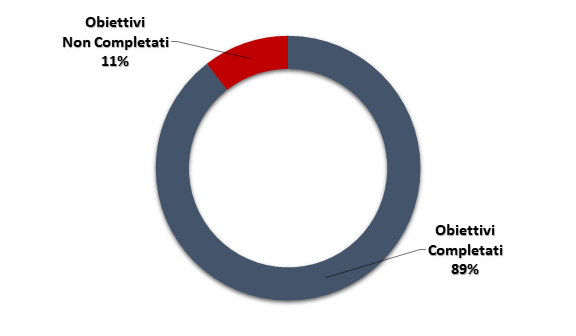
\includegraphics[width=0.5\textwidth]{immagini/Percentuale_Obiettivi_Completati}
	   	\caption{Percentuale completamento obiettivi di stage}
	   	%\vspace{2mm}
	\end{figure}

\subsection{Obiettivi personali}
%In questa sottosezione riporterò gli obiettivi personali che sono stati raggiunti.
Inizialmente, con l'inizio del percorso di stage, mi ero posto degli obiettivi, tali obiettivi sono stati parzialmente raggiunti. Con la soddisfacente richiesta dell'azienda di proseguire con i restanti quattro mesi di stage, infatti, ho raggiunto l'obiettivo più grande, ovvero proseguire sulla strada che portava verso la concretizzazione della mia ambizione.\\

Oltre a questo al termine del periodo di stage ero in grado di contribuire lato tecnico e potevo anche, seppur parzialmente, dare un contributo lato funzionale, su cui continuava il mio processo di apprendimento.

\section{Gap analysis}
%In questa sezione riporterò quelli che secondo me sono punti importanti che nel percorso accademico non vengono trattati ma che nel mondo del lavoro sono essenziali o dati per scontato.

Come accennato in varie sezioni le fondamenta di carattere tecnico che avevo all'inizio del percorso di stage hanno fatto sì che io sia produttivo senza particolari difficoltà. Il percorso di studi che ho intrapreso sin dall'inizio delle scuole superiori, infatti, è sempre stato di carattere formativo sul campo dell'informatica.\\

Con il percorso di studi all'interno dell'Università degli Studi di Padova, e precisamente con il Corso di Laurea Triennale in Informatica ho avuto modo di approfondire concetti informatici essenziali, arrivando alla conclusione di questo periodo formativo con le abilità e le competenze richieste dalla maggior parte delle aziende ICT.\\

Analizzando le conoscenze che la formazione accademica fornisce in relazione a quel che il mio stage richiedeva posso affermare che tale percorso è più che sufficiente.\\

In particolare i corsi che più mi sono serviti nel contesto aziendale sono stati: 
\begin{itemize}
	\item Il corso di Programmazione con l'insegnamento di quella che è la modalità di sviluppo procedurale;
	\item Il corso di Basi di Dati con l'insegnamento d'uso dei DBMS\glossario\ e del linguaggio SQL;
	\item Il corso di Ingegneria del Software con l'insegnamento relativo ai vari cicli di sviluppo.
\end{itemize}

Durante lo stage ho necessitato di concetti teorico-economici che durante il corso di studi non sono stati trattati, questo però è accettabile avendo seguito un Corso di Laurea in \textit{Informatica}.\\

Ritengo quindi che il corso prepari in modo più che sufficiente al mondo del lavoro e permetta di integrarsi in ambienti professionali che utilizzino anche linguaggi e tecnologie non trattate durante lo stesso.